Section \ref{C1-SubSection:Household-Responses-to-the-Lagged-Marginal-Prices} presents the empirical evidence that SMUD residential customers under IBP reduced their average daily electricity consumption in a billing cycle (i.e., in Period 1) as a response to the increase in the marginal price in the immediate previous billing period (i.e., in Period 0). In this section, I examine how their electricity consumption responded to the lagged price signals in a prolonged time interval---the relationship between Period $-1$ and Period 1 as well as Period $-2$ and Period 1. In other words, I study the impact of the lagged marginal price on household electricity consumption in two- and three-month intervals. Clearly, the conditions on which my RD design relies, which are described in Section \ref{C1-Sub-Sub-Section:Regression-Discontinuity-Design}, still hold in the multi-period setting here. Nevertheless, the seasonal variation in the lower base usage quantity might significantly alter households' consumption behavior over a longer time frame. To rule out this potential confounding factor, I focus on the summer and winter seasons, during which the cutoff point for each season remained at the same level. 

\afterpage{
    \begin{figure}[t!]
        \centering
        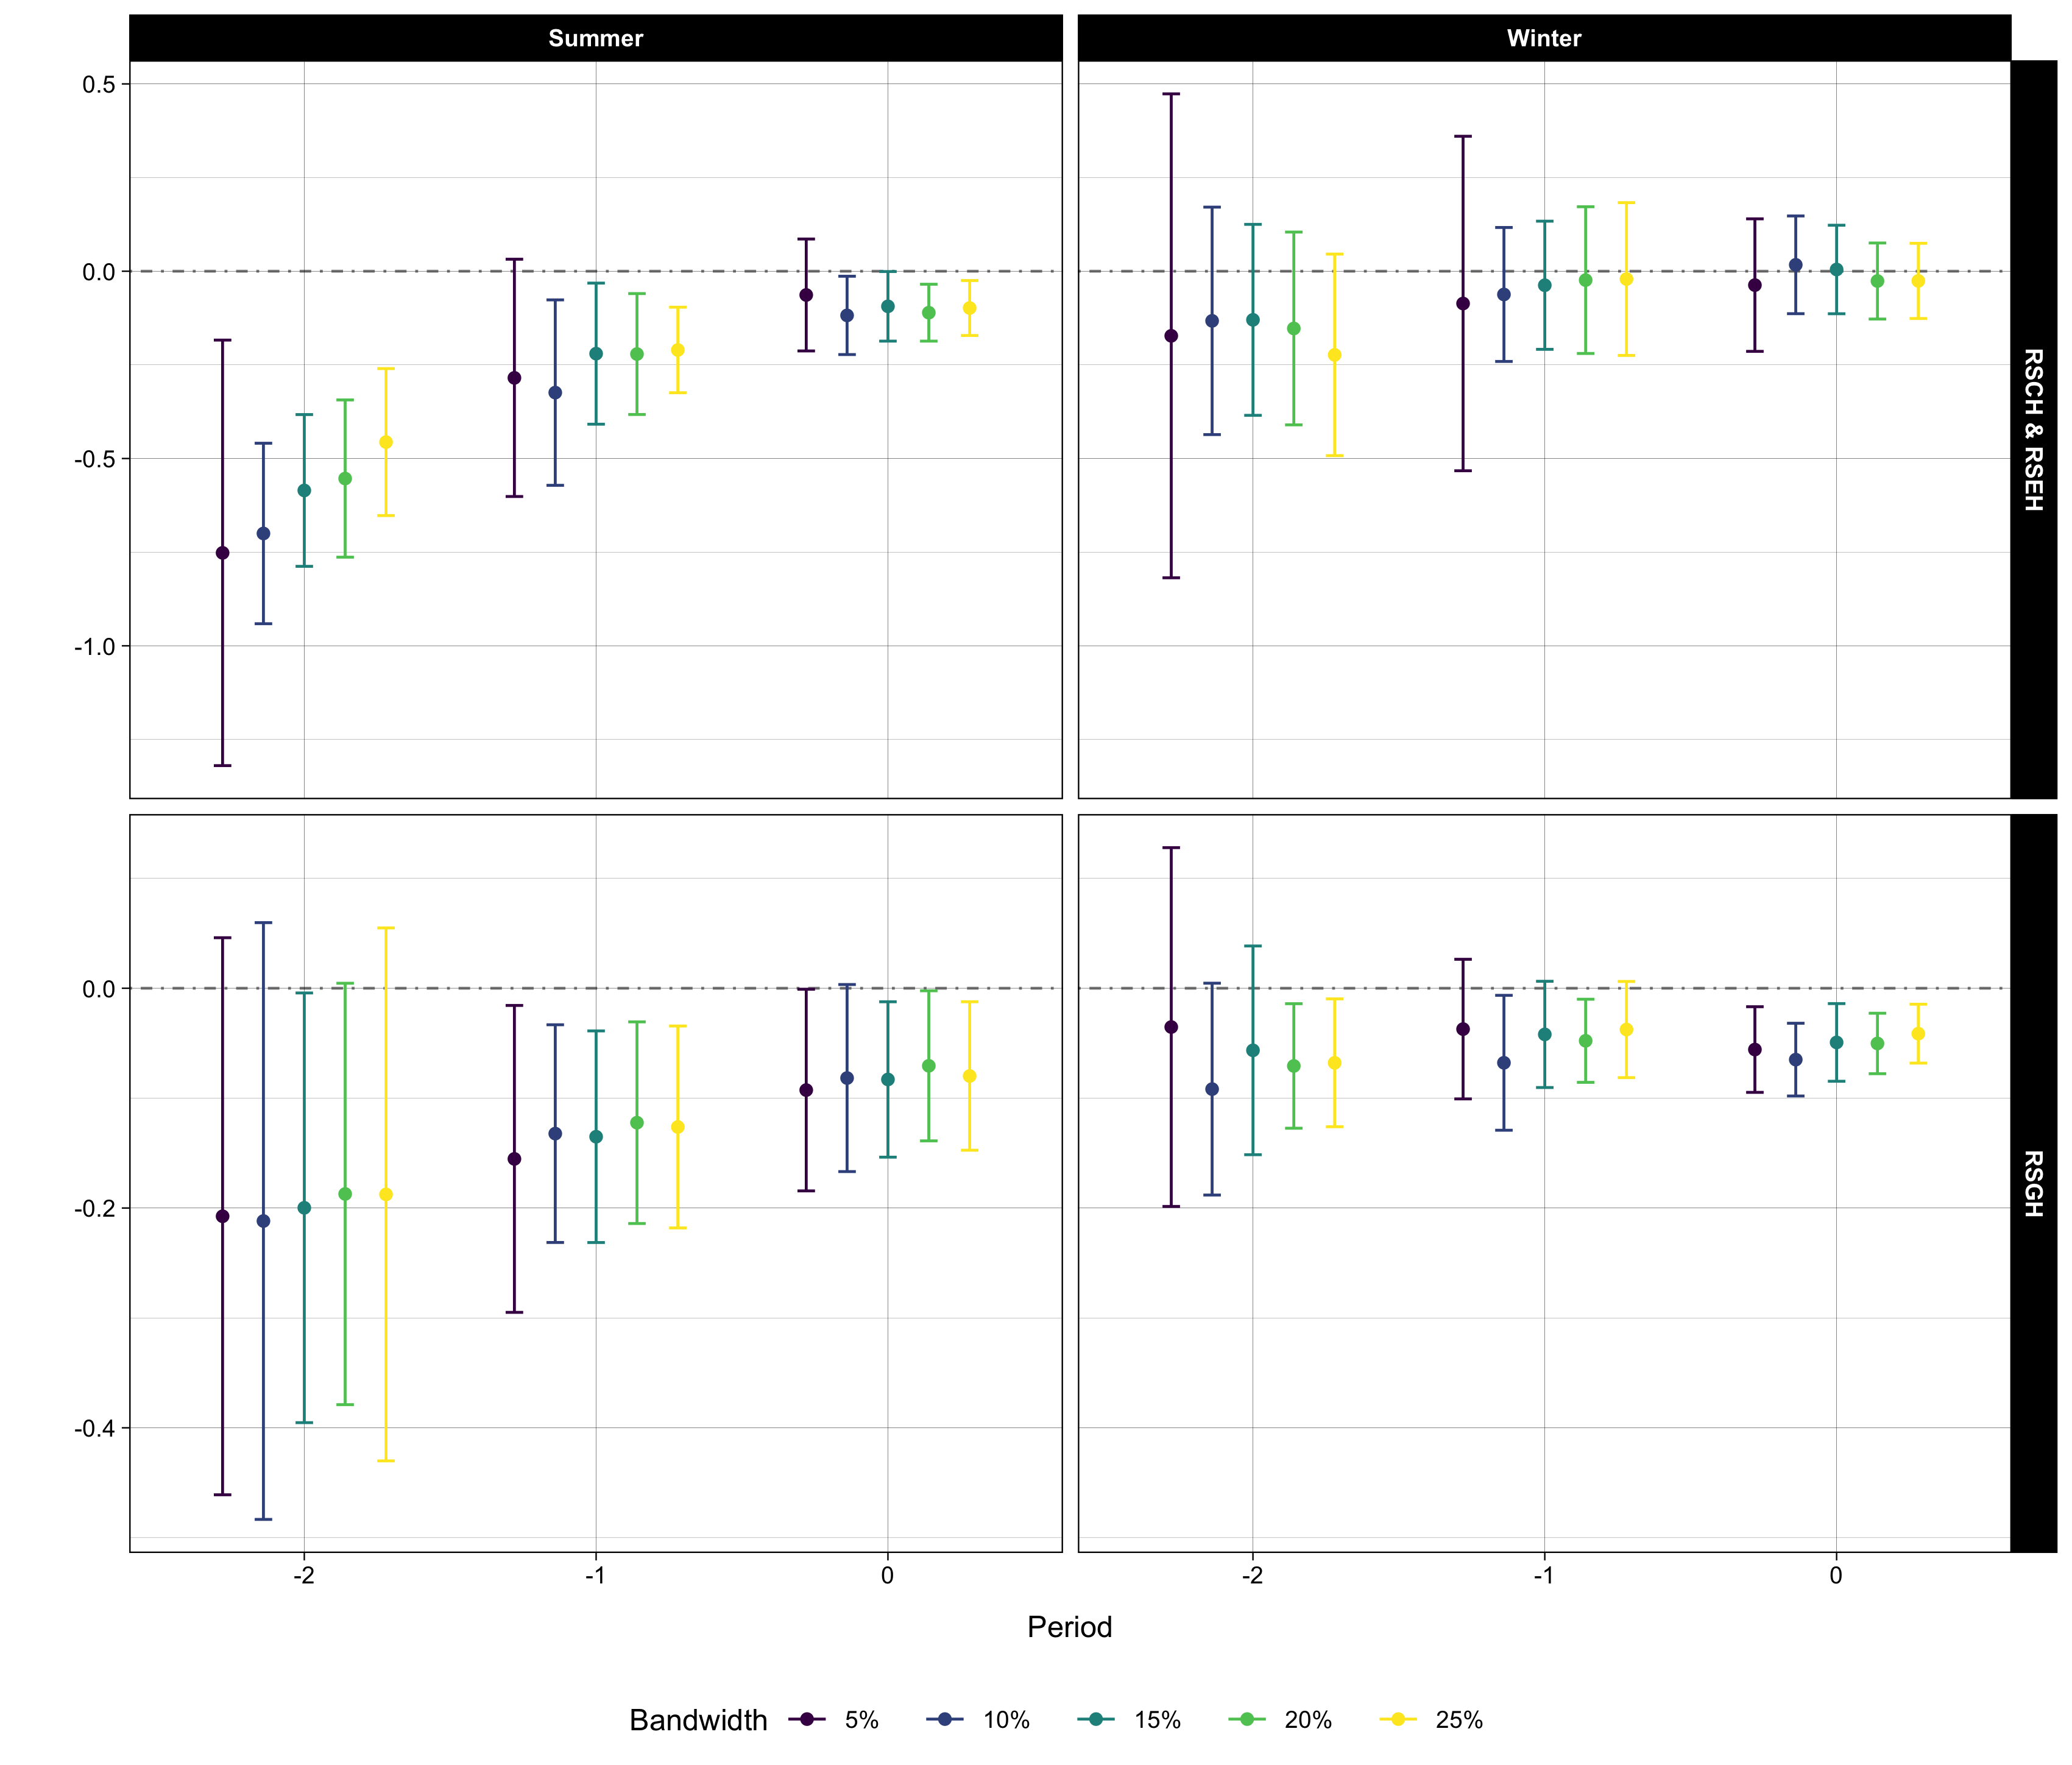
\includegraphics[scale = 0.133]{02_Chapter-1/00A_Figures/Figure_Multi-Period-Treatment-Effects_By-Season.png}
        \caption{Multi-Period Treatment Effects}
        \caption*{
            {\small
            \textit{Note}: 
            This figure summarizes the estimated multi-period treatment effects. The over-period evolving pattern of the estimates for electric-heating households (i.e., households selecting either the RSCH or RSEH rate plan) is significantly different from that of the estimates for non-electric-heating households (i.e., households choosing the RSGH rate code). See the text for details. 
        }}
        \label{Figure:Multi-Period-Treatment-Effects}
    \end{figure}
}
Figure \ref{Figure:Multi-Period-Treatment-Effects} shows the estimated multi-period treatment effects for a set of bandwidths. The two panels on the left side of this figure are for the summer season, whereas those on the right are for the winter season. The upper and lower panels present the estimated multi-period treatment effects for households with either one of the two electric-heating rate plans and those with the RSGH rate plan, respectively. 

The households choosing electric heating rate plans, whose base usage quantities moved together seasonally, demonstrated vastly different responses in the two seasons. In the summer season, they reacted to the discontinuous increases in the lagged marginal price by reducing their electricity consumption. Interestingly, the lagged price signals persisted over multiple billing cycles. Furthermore, their consumption reductions were more considerable for earlier price signals. In addition to the summer season's higher prices and much lower base usage quantity, the salience of Period $-2$'s winter-to-summer transition in marginal prices and base usage quantities, compared to Period $-1$ and Period 0, could affect their responsiveness to the lagged marginal price. As described in the upper right panel, the SMUD residential customers did not respond to the lagged price signals in the winter season. Similar to the no response in the higher base usage quantity, the significantly higher cutoff point at which the first discontinuous price jump occurred in the winter season may explain this response. 

In both seasons, the households selecting the RSGH rate plan showed similar responses. One notable point from their responses is that the marginal price's discontinuous increase in Period $-2$ had minimal impact on their electricity consumption in Period 1. In other words, the impact of the discontinuous increases on household electricity consumption tends to dissipate gradually over time.\footnote{The salience of the winter-to-summer transition, accompanying relatively small price increases and growths in base usage quantities, seems not to play an important role in altering households' consumption behavior.} 
